\documentclass[,a4paper]{article}
\usepackage{geometry}
\geometry{a4paper,left=35mm,right=35mm, top=25mm, bottom=25mm}
\usepackage[T1]{fontenc}
\usepackage{lmodern}
\usepackage{amssymb,amsmath}
\usepackage{ifxetex,ifluatex}
\usepackage{fixltx2e} % provides \textsubscript
% use microtype if available
\IfFileExists{microtype.sty}{\usepackage{microtype}}{}
\ifnum 0\ifxetex 1\fi\ifluatex 1\fi=0 % if pdftex
  \usepackage[utf8]{inputenc}
\else % if luatex or xelatex
  \usepackage{fontspec}
  \ifxetex
    \usepackage{xltxtra,xunicode}
  \fi
  \defaultfontfeatures{Mapping=tex-text,Scale=MatchLowercase}
  \newcommand{\euro}{€}
\fi
% Redefine labelwidth for lists; otherwise, the enumerate package will cause
% markers to extend beyond the left margin.
\makeatletter\AtBeginDocument{%
  \renewcommand{\@listi}
    {\setlength{\labelwidth}{4em}}
}\makeatother
\usepackage{enumerate}
\usepackage{graphicx}
% We will generate all images so they have a width \maxwidth. This means
% that they will get their normal width if they fit onto the page, but
% are scaled down if they would overflow the margins.
\makeatletter
\def\maxwidth{\ifdim\Gin@nat@width>\linewidth\linewidth
\else\Gin@nat@width\fi}
\makeatother
\let\Oldincludegraphics\includegraphics
\renewcommand{\includegraphics}[1]{\Oldincludegraphics[width=\maxwidth]{#1}}
\ifxetex
  \usepackage[setpagesize=false, % page size defined by xetex
              unicode=false, % unicode breaks when used with xetex
              xetex]{hyperref}
\else
  \usepackage[unicode=true]{hyperref}
\fi
\hypersetup{breaklinks=true,
            bookmarks=true,
            pdfauthor={Marian Steinbach marian@sendung.de},
            pdftitle={OParl Schnittstellen-Spezifikation (Entwurf)},
            colorlinks=true,
            urlcolor=blue,
            linkcolor=magenta,
            pdfborder={0 0 0}}
\setlength{\parindent}{0pt}
\setlength{\parskip}{6pt plus 2pt minus 1pt}
\setlength{\emergencystretch}{3em}  % prevent overfull lines
\setcounter{secnumdepth}{0}

\title{OParl Schnittstellen-Spezifikation (Entwurf)}
\author{Marian Steinbach
                \href{mailto:marian@sendung.de}{\texttt{marian@sendung.de}}}
\date{}

\begin{document}
\maketitle

Lizenz: Creative Commons CC-BY-SA

\section{Einleitung}

Dieses Dokument wird bei seiner Fertigstellung die Spezifikation des
OParl Schnittstellen-Standards für parlamentarische Informationssysteme
(Ratsinformationssysteme, RIS) darstellen. Es dient damit als Grundlage
für die Implementierung von OParl-konformen Server- und
Clientanwendungen.

\subsection{Parlamentarische Informationssysteme}

Parlamentarische Informationssysteme (oft Ratsinformationssystem, RIS
oder Bürgerinformationssystem genannt) werden von vielen Körperschaften
wie Kommunen, Landkreisen und Regierungsbezirken eingesetzt, um die
anfallende Gremienarbeit (Ratssitzungen, Ausschüsse, Vertretungen) zu
organisieren. Da ein großer Teil der schriftlichen Arbeit in der
Lokalpolitik über derartige Systeme verwaltet wird, sind diese Systeme
-- dort wo vorhanden -- ein wichtiger Zugriffspunkt für alle, die sich
für politischen Geschehnisse interessieren.

\subsection{Gründe für den standardisierten Datenzugriff}

Eine wichtige Maßnahme von Körperschaften, die im Zuge von Open-Data-
und Open-Government-Initiativen ihre Politik transparenter machen
wollen, wird auch sein, die Daten in den parlamentarischen
Informationssystemen im Sinne des Open-Data-Begriffs zugänglich zu
machen. Hierdurch können die Kommunen selbst, aber auch dritte,
Anwendungen entwickeln, die Inhalte auf verschiedene Art und Weise
auswerten, abrufbar und nutzbar machen, sei es für die Allgemeinheit
oder für bestimmte Nutzerkreise.

Darüber hinaus sollen parlamentarische Informationssysteme in
verschiedenste Prozesse und Systemlandschaften integriert werden. Durch
eine einheitliche Schnittstelle bieten sich effiziente Möglichkeiten zur
Integration der Daten in anderen Systemen, wie beispielsweise
Web-Portalen.

\subsection{Funktionsumfang der OParl-Schnittstelle}

Die vorliegende Spezifikation soll eine Webservice-Schnittstelle
definieren, die den anonymen und lesenden Zugriff auf öffentliche
Inhalte aus Parlamentarischen Informationssystemen ermöglicht. Die
Zugriffe erfolgen über das Hypertext Transfer Protocol (HTTP). Daten
werden als JSON, JSONP oder optional als XML ausgeliefert.

Die Spezifikation wird obligatorische Bestandteile (MUSS) und optionale
Bestandteile (KANN) haben. Der tatsächliche Funktionsumfang kann daher
zwischen den Implementierungen variieren.

\subsection{Status}

Die Spezifikation befindet sich in Arbeit. Das Dokument enthält
entsprechend viele Ungenauigkeiten und Hinweise auf offene
Fragestellungen.

\subsection{Überblick}

Der Entwurf umfasst aktuell die Beschreibung eines Datenmodells.

\subsection{Nächste Schritte}

Bis Ende Juni 2013: Fertigstellung von Version 1.0. Bis dahin ist zu
erledigen:

\begin{itemize}
\item
  Fertigstellung Datenmodell
\item
  Beschreibung von Methoden und URL-Parametern
\item
  HTTP Status-Codes und besondere Anforderungen an Verwendung bestimmter
  HTTP-Header
\item
  Klärung einer gemeinsamen Nomenklatur für Inhalte, beispielsweise für
  Arten von Drucksachen
\end{itemize}

\subsection{Feedback und Mitwirkung}

Feedback wird dringend benötigt und ist daher herzlichst willkommen.
Feedback kann auf den folgenden Wegen eingereicht werden:

\begin{itemize}
\item
  Als Pull Requests über Github, direkt am Quelltext
\item
  Über Issues auf Github
\item
  Per E-Mail
\end{itemize}

\subsubsection{Pull Requests über Github}

Dieses Dokument wird in folgendem Github-Repository gepflegt:

\href{https://github.com/OParl/specs}{https://github.com/OParl/specs}

Der bevorzugte Feedback-Kanal für erfahrene Git- bzw. Github-Nutzer ist
entsprechend die Mitwirkung direkt am Quelltext in Form von
Pull-Requests. So können \textbf{Ergänzungen und Korrekturen} direkt in
den Quelltext eingespielt werden.

Ausführliche Anleitungen zur Arbeit mit Git/Github finden sich auf der
Plattform selbst sowie an vielen Orten im Netz. Der allgemeine Ablauf
ist wie folgt:

\begin{enumerate}[1.]
\item
  Erzeugen Sie sich, sofern noch nicht geschehen, ein Benutzerkonto auf
  Github.
\item
  Duplizieren (\emph{forken}) Sie das oben genannte Repository
\item
  Nehmen Sie die gewünschten Änderungen an Ihrem Repository vor.
  Committen Sie diese Änderungen möglichst kleinteilig.
\item
  Senden Sie die gewünschten Commits als Pull Requests.
\end{enumerate}

Als Autor werde ich entscheiden, welche Pull Requests ich übernehme. Sie
werden als Mitwirkender in diesem Dokument genannt. Wenn Sie mit einen
Klarnamen unggf. Unternehmenszugehörigkeit genannt werden wollen, teilen
Sie mir dies bitte per Mail an marian@sendung.de mit.

\subsubsection{Issues auf Github}

Wer nicht über Github am Quelltext mitwirken möchte, aber einen
Github-Account sein eigen nennt (oder zu diesem Zweck anlegen möchte)
und \textbf{öffentlich kommentieren} möchte, der sollte das öffentliche
Issue-Tracking-System unter

\href{https://github.com/OParl/specs/issues}{https://github.com/OParl/specs/issues}

verwenden. Vorteil daran ist, dass auch andere die Einträge lesen und
wiederum durch Kommentare ergänzen können. Zudem lässt sich der
Bearbeitungsstatus eines Issue-Eintrags (offen, geschlossen) nachhalten.

Bitte achten Sie auf diesem Weg darauf, Ihre Kommentare in möglichst
kleine thematische Einheiten herunter zu brechen.

\subsubsection{Feedback per E-Mail}

Sollten Sie keinen der oben beschriebenen Wege beschreiten wollen,
können Sie Anmerkungen zum Dokument per E-Mail an marian@sendung.de
einsenden. Bitte verwenden Sie dabei den Begriff ``oparl-specs'' im
Betreff.

Sollten Sie auf diesem Wege Anmerkungen direkt am/im Dokumententext
übersenden wollen, nutzen Sie bitte falls möglich die Word- oder
OpenOffice-Version dieses Dokuments und ändern Sie das Dokument so, dass
Änderungen aufgezeichnet werden (OpenOffice: Bearbeiten \textgreater{}
Änderungen \textgreater{} Aufzeichnen; Word: Ribbon ``Überprüfen''
\textgreater{} Nachverfolgung \textgreater{} Änderungen nachverfolgen).

\subsection{Mitwirkende}

Felix Ebert, Jan Erhardt, Andreas Kuckartz, Babett Schalitz

\section{Datenmodell}

Das Datenmodell definiert die Objekttypen bzw. die Klassen, auf die über
die Schnittstelle zugegriffen werden kann.

Die Hinweise auf die Praxis in bestehenden Ratsinformationssystemen
beziehen sich auf nach außen, bei Nutzung der jeweiligen Weboberflächen,
feststellbare Eigenschaften. Dabei wird vereinzelt und beispielhaft auf
die folgenden Systeme Bezug genommen:

\begin{itemize}
\item
  Stadt Köln {[}2{]} - Plattform: Somacos SessionNet {[}3{]}
\item
  Bezirksverwaltung Berlin Mitte {[}4{]} - Plattform: ALLRIS {[}5{]}
\item
  Stadt Rösrath {[}6{]} - Plattform der Firma PROVOX {[}7{]}
\item
  Stadt Euskirchen {[}8{]} - Plattform: SD.NET RIM 4 {[}9{]}
\item
  Stadt Bonn - BoRis {[}10{]}
\end{itemize}

\subsection{Übergreifende Aspekte}

\subsubsection{Eindeutige Identifizierung von Objekten}

Sämtliche Objekte, die über die Schnittstelle geladen werden können,
sollen anhand einer einzigen Objekteigenschaft eindeutig identifizierbar
sein. Die Objekteigenschaft, mit der dies erreicht wird, wird hier im
folgenden - unabhängig vom tatsächlichen Namen der Eigenschaft - als
``Schlüssel'' bezeichnet.

Eindeutigkeit meint hier eine Einzigartigkeit innerhalb des
Informationssystems und für den jeweiligen Objekttyp. Das bedeutet: zwei
von einander unabhängige Ratsinformationssysteme für verschiedene
Körperschaften dürfen sich überlappende Schlüssel nutzen. Innerhalb
eines Systems dürfen zwei Objekte unterschiedlichen Typs (beispielsweise
eine Person ud ein Gremium) den selben Schlüssel nutzen. Jedoch MÜSSEN
zwei Objekte des selben Typs innerhalb des selben Systems grundsätzlich
verschiedene Schlüssel haben.

Schlüssel-Eigenschaften werden grundsätzlich als String mit
Unicode-Zeichenumfang übergeben. Sie können daher gleichermaßen aus
numerischen wie alphanumerischen Werten befüllt werden.

Es wird grundsätzlich vorausgesetzt, dass Schlüssel unveränderlich sind.
Ändert sich der Schlüssel eines Objekts nach der Erzeugung, werden
Nutzer der Schnittstelle annehmen, dass es sich nicht mehr um das selbe
Objekt handelt.

\subsubsection{Objekteigenschaften}

Die nachfolgend beschriebenen Eigenschaften der Objekttypen sind, wenn
nicht anders angegeben, verpflichtend. Das bedeutet: Bei jedem von der
Schnittstelle ausgelieferten Objekt muss diese Eigenschaften definiert
sein. Optionale Eigenschaften sind entsprechend gekennzeichnet.

Eigenschaften werden deutschsprachig und englischsprachig benannt. Die
deutschsprachige Benennung dient der bestmöglichen Verständlichkeit im
Kontext dieses Dokuments, während die Schnittstelle aus Gründen der
Zugänglichkeit für möglichst viele Entwickler mit englischsprachigen
Begriffen arbeiten soll.

\subsubsection{Zu den Beziehungen}

Bei der Beschreibung von Beziehungen zwischen Objekten wird zu diesem
Zeitpunkt nicht berücksichtigt, ob eine Beziehung zwischen zwei Objekten
A und B am Objekt A oder am Objekt B definiert wird. So spielt es
bislang keine Rolle, ob einem Gremium mehrere Personen zugeordnet werden
oder einer Person mehrere Gremien zugewiesen werden. Das Augenmerkt
liegt hier nur auf der Tatsache, welche Beziehung existieren können und
was diese Beziehungen aussagen sollen.

\subsection{Körperschaft (\emph{body})}

Die Körperschaft erlaubt es, den Betreiber bzw. Eigentümer des
Informationssystems wie zum Beispiel einen Landkreis, eine bestimmte
Gemeinde oder einen bestimmten Stadtbezirk in Form eines Datenobjekts
abzubilden.

Viele RIS werden nur genau eine Instanz dieses Typs „beherbergen``.
Einige Systeme werden jedoch für mehrere Mandanten betrieben, wobei die
Mandanten verschiedene Körperschaften repräsentieren
(z.B.''Verbandsgemeinde Ulmen" und ``Stadt Ulmen''.)

\begin{figure}[htbp]
\centering
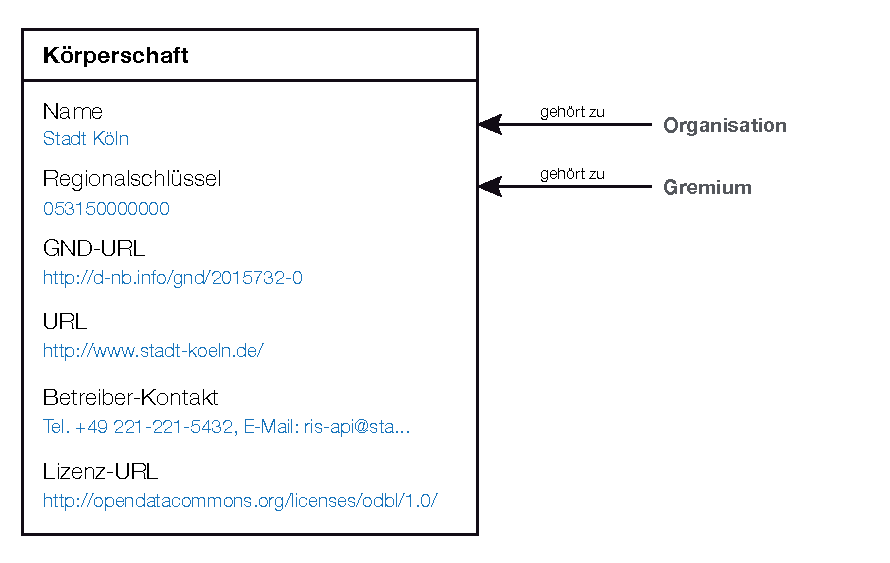
\includegraphics{images/datenmodell_koerperschaft.pdf}
\caption{Objekttyp Körperschaft}
\end{figure}

\subsubsection{Eindeutige Identifizierung}

Zur Identifizierung des Objekts kann der Amtliche Gemeindeschlüssel
(AGS{[}1{]}) verwendet werden, der alle deutschen Gemeinden, Landkreise,
kreisfreien Städte etc. eindeutig erfasst.

Vorteil der Verwendung des AGS:

\begin{itemize}
\item
  Kompakte, einfache und einheitliche Schreibweise für jede
  Körperschaft.
\item
  Der AGS wird von Behörden genutzt, ist anerkannt und auch in anderen
  Medien, z.B. der Wikipedia, verbreitet.
\end{itemize}

Nachteil des AGS:

\begin{itemize}
\item
  Führende Nullen machen den Schlüssel fehleranfällig. Bestimmte Systeme
  wie z.B. Excel könnten den Inhalt als Zahlenwert erkennen und die
  führenden Nullen automatisch verwerfen.
\item
  Für Gebietsgliederungen unterhalb der selbstständigen Gemeinde,
  beispielsweise einen einzelnen Stadtbezirk, gibt es keinen eigenen
  Gemeindeschlüssel. Dies müssten durch eine nicht-amtliche Erweiterung
  des Systems ausgeglichen werden.
\end{itemize}

\subsubsection{Eigenschaften}

\begin{description}
\item[Name]
Der Name der Körperschaft, z.B. ``Köln'' oder ``Stadt Köln''.
\end{description}

\subsubsection{Beziehungen}

\begin{itemize}
\item
  Objekte vom Typ ``Organisation'' sind zwingend genau einer
  Körperschaft zugeordnet. So wird beispielseise eine SPD in Köln von
  einer SPD in Leverkusen unterschieden.
\item
  Objekte vom Typ ``Gremium'' sind zwingend genau einer Körperschaft
  zugeordnet. Damit wird der ``Rat'' einer bestimmten Kommune von den
  gleichnamigen Gremien anderer Kommunen abgegrenzt.
\end{itemize}

\subsection{Gremium (\emph{committee})}

Das Gremium ist ein Personenkreis, üblicherweise von gewählten und/oder
ernannten Mitgliedern. Beispiele hierfür sind der Stadtrat, Kreisrat,
Gemeinderat, Ausschüsse und Bezirksvertretungen. Gremien halten
Sitzungen ab, zu denen die Gremien-Mitglieder eingeladen werden.

\begin{figure}[htbp]
\centering
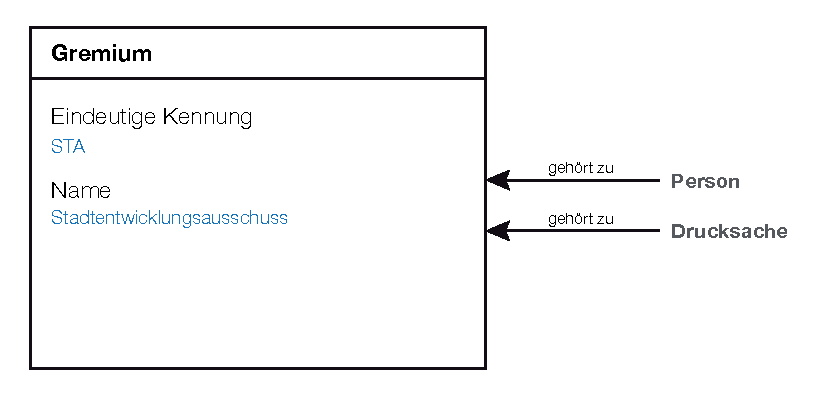
\includegraphics{images/datenmodell_gremium.pdf}
\caption{Objekttyp Gremium}
\end{figure}

\subsubsection{Eigenschaften}

\begin{description}
\item[Kennung]
Zur eindeutigen Identifizierung des Gremiums im Kontext einer bestimmten
\end{description}

Körperschaft. In der Praxis kommen sowohl numerische IDs als auch
Namenskürzel (Beispiel: ``STA'' für den Stadtentwicklungsausschuss) vor.
Beides sollte hier Verwendung finden können. Name : Der Name des
Gremiums. Beispiele: ``Rat'', ``Hauptausschuss'', ``Bezirksvertretung 1
(Innenstadt)'' Kurzname : \emph{Optional}. Eine zur Anzeige bestimmte,
kürzere Form des Namens.

\subsubsection{Beziehungen}

\begin{itemize}
\item
  Objekte vom Typ ``Person'' referenzieren auf Gremien, um die
  Mitgliedschaft/Zugehörigkeit einer Person im/zum Gremium zu
  kennzeichnen. Diese Beziehung ist datiert. Das bedeutet, sie hat einen
  Anfangszeitpunkt und ggf. einen Endzeitpunkt.
\item
  Objekte vom Typ ``Drucksache'' verweisen auf Gremien. Beispielsweise
  wird eine Anfrage oder ein Antrag dem Rat und/oder einer bestimmten
  Bezirksvertretung zugeordnet. Details zu dieser Beziehung werden unter
  ``Drucksache'' erläutert.
\end{itemize}

\subsection{Person (\emph{person})}

Jede natürliche Person, die Mitglied eines Gremiums ist, ist als Person
im Datenmodell eindeutig identifizierbar.

\begin{figure}[htbp]
\centering
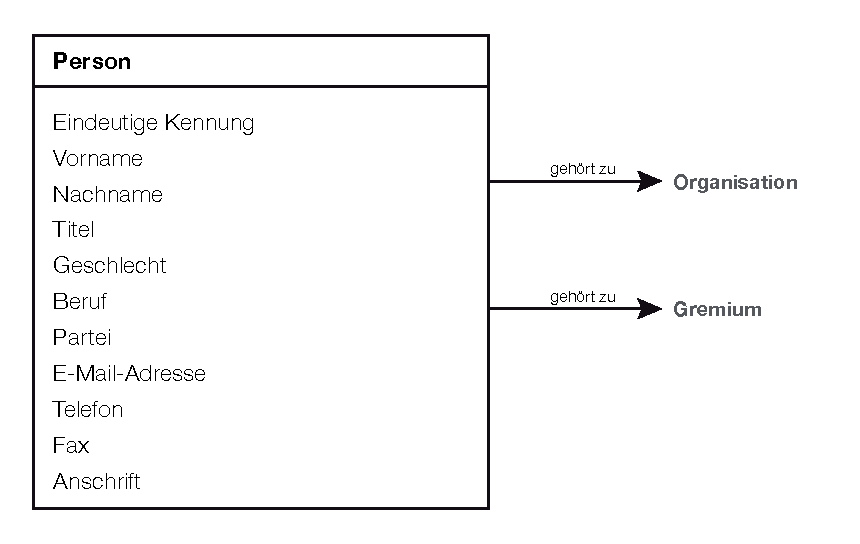
\includegraphics{images/datenmodell_person.pdf}
\caption{Objekttyp Person}
\end{figure}

\subsubsection{Eigenschaften}

\begin{description}
\item[Kennung]
Zur eindeutigen Identifizierung sollte jede Person eine Kennung
besitzen,
\end{description}

die keinen Änderungen unterworfen ist und aus diesem Grund nicht mit dem
Namen in Verbindung stehen sollte. Viele RIS nutzen rein numerische
Kennungen. Vorname : Der Vorname der Person. Nachname : Der Nachname der
Person. Titel : \emph{Optional}. Akademische Titel wie ``Dr.'' und
``Prof.~Dr.'' Geschlecht : \emph{Optional}. Männlich/Weblich Beruf :
\emph{Optional}. Z.B. ``Rechtsanwalt'' Partei : \emph{Optional}. Z.B.
``Bündnis 90/Grüne'' E-Mail-Adresse : \emph{Optional}. Telefon :
\emph{Optional}. Fax : \emph{Optional}. Anschrift : \emph{Optional}.
Straße und Hausnummer, Postleitzahl und Ort

\paragraph{Anmerkungen}

\begin{itemize}
\item
  Das System von Euskirchen scheint Vor- und Nachname (evtl. einschl.
  Titel) in einem gemeinsamen Feld ``Name'' zu führen. Ob das System
  hier technisch differenziert, ist unklar. Falls einzelne Systeme den
  angezeigten Namen nur als ganzes speichern, sollte dies für den
  Standard übernommen werden, da es für die meisten Anwendungen
  ausreichen sollte.
\item
  Das System PROVOX unterscheidet zwischen privaten und geschäftlichen
  Anschriften.
\end{itemize}

\subsubsection{Beziehungen}

\begin{itemize}
\item
  Objekte vom Typ ``Person'' können einer Organisation, z.B. einer
  Fraktion, zugeornet werden. Diese Beziehung ist datiert.
\item
  Objekte vom Typ ``Person'' können einem oder mehreren Gremien
  zugewiesen werden, um die Mitgliedschaft in diesem Gremium
  darzustellen. Diese Beziehungen sind ebenfalls datiert.
\end{itemize}

\subsection{Organisation (\emph{organisation})}

Organisationen sind üblicherweise Parteien bzw. Fraktionen, denen die
Personen angehören können.

\begin{figure}[htbp]
\centering
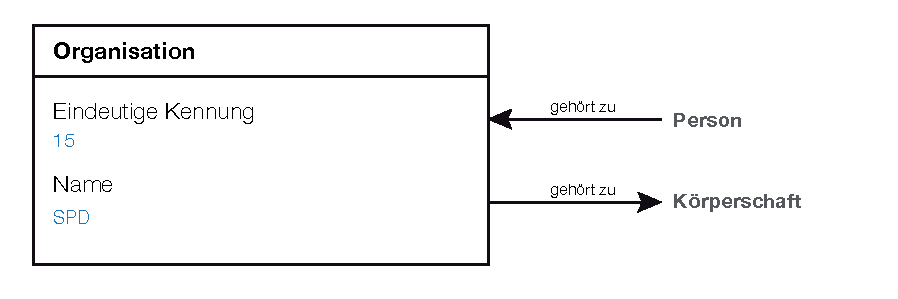
\includegraphics{images/datenmodell_organisation.pdf}
\caption{Objekttyp Organisation}
\end{figure}

\subsubsection{Eigenschaften}

\begin{description}
\item[Kennung]
Zur eindeutigen Kennzeichnung einer Organisation innerhalb einer
\end{description}

Körperschaft Name : Der gebräuchliche Name der Organisation, z.B.
``SPD'' oder ``DIE LINKE''.

\paragraph{Anmerkungen}

\begin{itemize}
\item
  Unklar ist bislang, ob Organisationen in der Praxis eher Fraktionen
  (``SPD-Fraktion im Kölner Rat'', ``SPD-Fraktion in Köln-Innenstadt'')
  abbilden oder ob eher Ortsverbände von Parteien (``SPD Köln'') gemeint
  sein werden. Einblicke, wie gängige Systeme dies handhaben, sollten
  evtl. gesammelt und berücksichtigt werden.
\end{itemize}

\subsubsection{Beziehungen}

\begin{itemize}
\item
  Jede Organisationen gehört zu einer Körperschaft.
\item
  Personen können Organisationen angehören (\emph{datiert}).
\end{itemize}

\subsection{Sitzung (\emph{meeting})}

Eine Sitzung ist die Versammlung der Mitglieder eines Gremiums oder
mehrerer Gremien zu einem bestimmten Zeitpunkt an einem bestimmten Ort.

Die geladenen Teilnehmer der Sitzung sind jeweils als „Person`` in
entsprechender Form referenziert. Verschiedene Dokumente (Einladung,
Ergebnis- und Wortprotokoll, sonstige Anlagen) können referenziert
werden.

\begin{figure}[htbp]
\centering
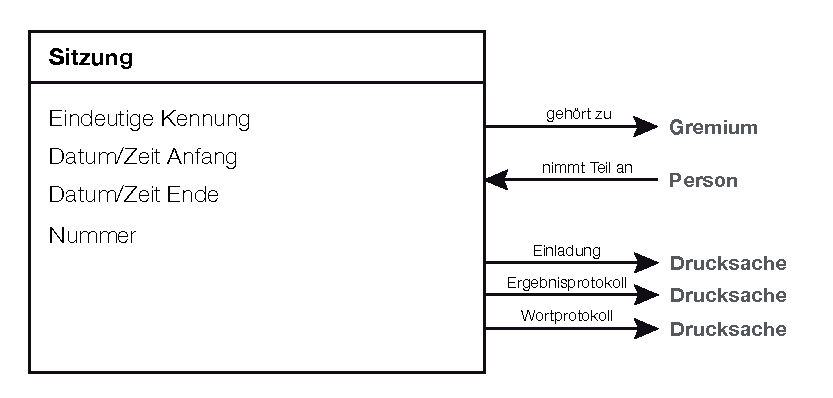
\includegraphics{images/datenmodell_sitzung.pdf}
\caption{Objekttyp Sitzung}
\end{figure}

\subsubsection{Eigenschaften}

\begin{description}
\item[Eindeutige Kennung]
Zur eindeutigen Identifizierung der Sitzung innerhalb einer
\end{description}

Körperschaft. In der Praxis wird eine solche Kennzeichnung entweder
durch eine laufende Nummer gebildet, oder durch Kombination mehrerer
Merkmale wie dem Kürzel des Gremiums, der laufenden Nummer der Sitzung
in einem Jahr und der Jahreszahl (z.B. ``BV1/0034/2012''). Nummer :
\emph{Optional}. Laufende Nummer der Sitzung, üblicherweise innerhalb
der Wahlperiode mit 1 beginnend. In der Praxis wird dadurch z.B. die
``2. Sitzung des Rats'' gekennzeichnet. Anfang : Datum und ggf. Uhrzeit
des Anfangszeitpunkts der Sitzung Ende : \emph{Optional}. Datum und
Uhrzeit vom Ende der Sitzung Ort : \emph{Optional}. Textliche
Information zum Ort der Sitzung, z.B. ``Rathaus, Raum 136''.

\subsubsection{Beziehungen}

\begin{itemize}
\item
  Sitzungen sind mindestens einem Gremium zugeordnet
\item
  Einer Sitzung sind Personen zugeordnet, um die Teilnahme an der
  Sitzung auszudrücken.
\item
  Dokumente können vom Typ ``Sitzung'' \emph{optional} zu mehreren
  Zwecken referenziert werden:

  \begin{itemize}
  \item
    Zum Verweis auf die Einladung zur Sitzung
  \item
    Zum Verweis auf das Ergebnisprotokoll zur Sitzung
  \item
    Zum Verweis auf das Wortprotokoll zur Sitzung
  \end{itemize}
\item
  Weiterhin können Sitzungen beliebige weitere Dokumente, die keine
  eigenständigen Drucksachen sind, referenzieren. Dabei handelt es sich
  dann um nicht weiter spezifizierte Anlagen.
\end{itemize}

\subsection{Tagesordnungspunkt (\emph{agendaitem})}

Der Tagesordnungspunkt wird für eine bestimmte Sitzung angelegt, erhält
eine (innerhalb dieser Sitzung eindeutige) Nummer und einen Titel
(Betreff). Nach der Sitzung wird dem Tagesordnungspunkt außerdem ein
Ergebnis angehängt. Unter Umständen kann dem Tagesordnungspunkt ein
bestimmter Beschlusstext beigefügt sein. Sofern das Abstimmungsergebnis
nicht einstimmig ist, kann es durch mehrere referenzierende
``Stimmabgaben'' festgehalten werden.

Überlicherweise haben Sitzungen mehrere Tagesordnungspunkte.

\begin{figure}[htbp]
\centering
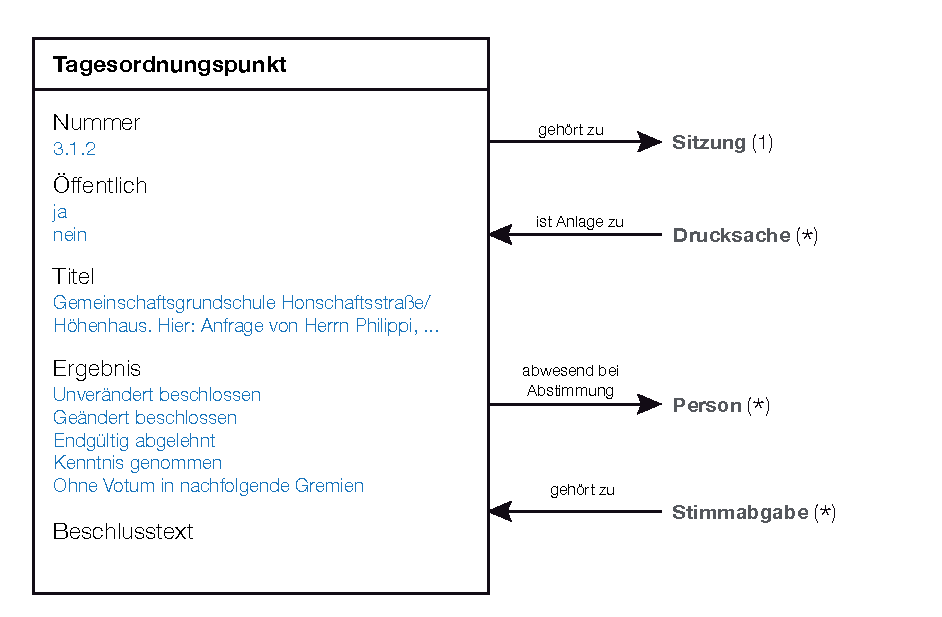
\includegraphics{images/datenmodell_tagesordnungspunkt.pdf}
\caption{Objekttyp Tagesordnungspunkt}
\end{figure}

\subsubsection{Eigenschaften}

\begin{description}
\item[Nummer]
Beispiel: ``1.2.3''. Diese Nummer gibt an, in welcher Reihenfolge die
\end{description}

Tagesordnungspunkte einer Sitzung normalerweise behandelt werden. Im
Kontext einer Sitzung ist diese Nummer eindeutig. Öffentlich : ja/nein.
Kennzeichnet, ob der Tagesordnungspunkt in öffentlicher Sitzung
behandelt wird. Titel : Das Thema des Tagesordnungspunktes Ergebnis :
Eines aus einer Liste definierter Ergebnisse. Möglich sind:
``Unverändert beschlossen'', ``Geändert beschlossen'', ``Endgültig
abgelehnt'', ``Zur Kenntnis genommen'', ``Ohne Votum in nachfolgende
Gremien überwiesen'' Beschlusstext : \emph{Optional}. Falls in diesem
Tagesordnungspunkt ein Beschluss gefasst wurde, kann der Text hier
hinterlegt werden. Das ist besonders dann in der Praxis relevant, wenn
der gefasste Beschluss (z.B. durch Änderungsantrag) von der
Beschlussvorlage abweicht.

\paragraph{Anmerkungen}

\begin{itemize}
\item
  Einige Systeme vergeben zu Tagesordnungspunkten intern
  unveränderliche, numerische IDs. Es ist unklar, ob es zusätzlichen
  Nutzen bringt, derartige IDs, neben den Nummern, in den Standard zu
  übernehmen. Dies würde vermutlich nur Sinn ergeben, wenn es als
  Pflichtfeld gelten kann.
\end{itemize}

\subsubsection{Beziehungen}

\begin{itemize}
\item
  Jeder Tagesordnungspunkt gehört zu genau einer Sitzung.
\item
  Der Tagesordnungspunkt kann auf eine Drucksache verweisen, die im
  Rahmen dieses Tagesordnungspunkt beraten werden soll.
\item
  Es können mehrere Objekte vom Typ ``Stimmabgabe'' referenziert werden,
  um das Abstimmungsverhalten von Fraktionen oder Einzelpersonen zu
  dokumentieren.
\item
  Es können Personen referenziert werden, die während der Abstimmung zu
  diesem Tagesordnungspunkt \emph{nicht} anwesend waren.
\end{itemize}

\subsection{Stimmabgabe (\emph{vote})}

Wie eine Person bzw. eine Fraktion zu einem Tagesordnungspunkt
abgestimmt hat, wird durch eine Stimmabgabe festgehalten. Ganze
Abstimmungsergebnisse bestehen überlicherweise aus mehreren
Stimmabgaben. Jede Stimmabgabe gibt entweder die (einzelne) Stimme einer
Peson wieder, in diesem Fall ist die Anzahl der Stimmen zwingend 1. Oder
eine Stimmabgabe gibt das Abstimmungsverhalten einer ganzen Gruppe von
Personen wieder. Dann ist die Anzahl der Stimmen anzugeben und statt
einer Person eine Organisation (in der Regel die Fraktion) zu
referenzieren.

\begin{figure}[htbp]
\centering
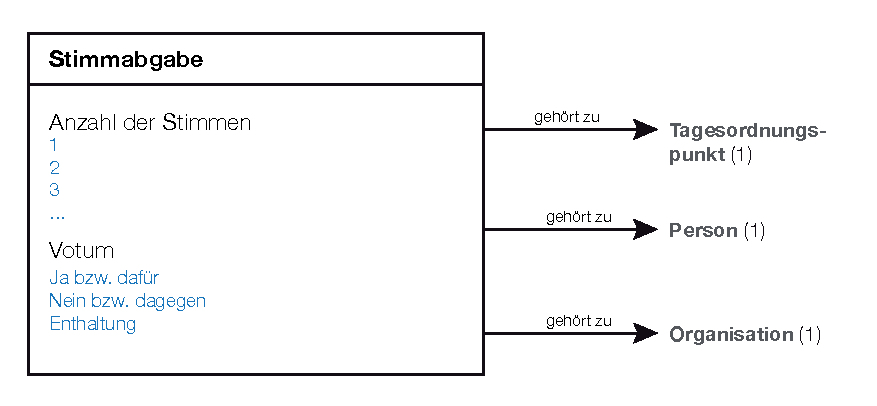
\includegraphics{images/datenmodell_stimmabgabe.pdf}
\caption{Objekttyp Stimmabgabe}
\end{figure}

\subsubsection{Eigenschaften}

\begin{description}
\item[Anzahl der Stimmen]
Gehört die Stimmabgabe zu einer Person, ist der Wert immer 1. Gehört sie
\end{description}

jedoch zu einer Organisation (=Fraktion), kann der Wert hier größer als
1 sein. Votum : Einer der drei Werte ``ja'' (gleichbedeutend mit
``dafür''), ``nein'' (``dagegen'') oder ``Enthaltung''.

\subsubsection{Beziehungen}

\begin{itemize}
\item
  Jede Stimmabgabe gehört zu genau einem Tagesordnungspunkt.
\item
  Es wird entweder genau eine Person oder genau eine Organisation
  (Fraktion) referenziert, die die Stimme(n) abgegeben hat.
\end{itemize}

\subsection{Drucksache (\emph{paper})}

Eine Drucksache bildet Mitteilungen, Antworten auf Anfragen,
Beschlussvorlagen, Anfragen und Anträge ab. Jede Drucksache erhält eine
eindeutige Kennung.

Die Drucksache hat im Informationsmodell eine hervorgehobene Bedeutung.
Im Fall eines Antrags kann mit einer einzigen Drucksache ein über Monate
oder Jahre dauernder politischer Entscheidungsprozess verbunden sein. In
dem Zusammenhang entstehen üblicherweise weitere Drucksachen.

Drucksachen spielen in der schriftlichen wie mündlichen Kommunikation
eine besondere Rolle, da in vielen Texten auf bestimmte Drucksachen
Bezug genommen wird. Hierbei kommen in Ratsinformationssystemen
unveränderliche Kennungen der Drucksachen zum Einsatz.

\begin{figure}[htbp]
\centering
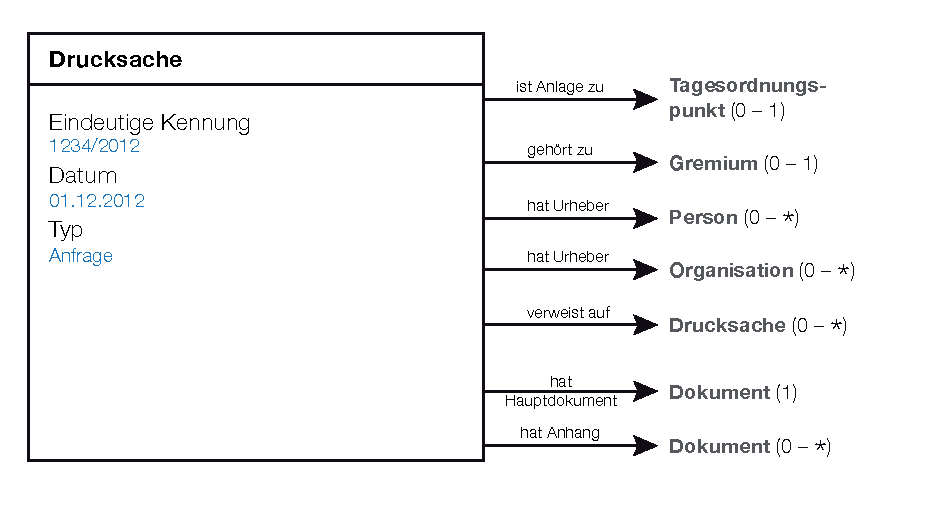
\includegraphics{images/datenmodell_drucksache.pdf}
\caption{Objekttyp Drucksache}
\end{figure}

Jede Drucksache ist über die Eigenschaft ``Typ'' als eine der folgenden
Arten von Drucksachen gekennzeichnet:

\begin{itemize}
\item
  \textbf{Beschlussvorlage}: Entscheidungsvorschlag der Verwaltung
\item
  \textbf{Antrag}: Entscheidungsvorschlag einer Fraktionen bzw. mehrerer
  Fraktionen oder einer/mehrerer Einzelperson/en
\item
  \textbf{Anfrage}: Frage(n) einer oder mehrerer Fraktion oder
  Einzelpersonen an die Verwaltung
\item
  \textbf{Mitteilung/Stellungnahme der Verwaltung}: Eine Information der
  Verwaltung an einzelne oder mehrere Gremien. Darunter fallen nicht
  Beantwortungen von Anfragen.
\item
  \textbf{Beantwortung einer Anfrage}: Antwort der Verwaltung auf
  (mündliche oder schriftliche) Anfragen
\end{itemize}

\subsubsection{Eigenschaften}

\begin{description}
\item[Kennung]
Die Kennung einer Drucksache muss für die jeweilige Körperschaft
\end{description}

eindeutig sein. Sie kann sowohl Ziffern als auch Buchstaben enthalten.
Einige Systeme (z.B. Köln) verwenden besondere Trennzeichen wie ``/'',
um eine Jahreszahl von einer laufenden Nummer abzutrennen. Weiterhin
werden mancherorts führende Nullen verwendet. Datum : Datum der
Veröffentlichung Typ : Art der Drucksache (Erläuterung siehe oben)

\subsubsection{Beziehungen}

\begin{itemize}
\item
  Es muss genau ein \textbf{Hauptdokument} (Objekttyp ``Dokument'')
  referenziert werden.
\item
  Es können beliebig viele weitere Dokumente referenziert werden, die
  als nachgeordnete \textbf{Anlagen} zur Drucksache verstanden werden.
\item
  Die Drucksache ist beliebig vielen Gremien zuzuordnen, in denen diese
  beraten wird.
\item
  Drucksachen können \textbf{Urhebern} zugewiesen werden. Im Fall von
  Mitteilungen der Verwaltung ist dies oft der Oberbürgermeister. Bei
  Anträgen oder Anfragen können Organisationen oder Einzelpersonen
  referenziert werden. Es können stets mehrere Uhrheber verknüpft
  werden.
\item
  Es können beliebig viele \textbf{Orte} (siehe Objekttyp ``Ort'')
  referenziert werden, die im Inhalt der Drucksache behandelt werden.
  Beispiel: Beschlussvorlage zur Freigabe von Mitteln für die Sanierung
  eines Sportplatzes, wobei der Ort die Lage des Sportplatzes genau
  beschreibt.
\item
  Drucksachen können auf andere Drucksachen referenzieren. Diese
  Verweise können verschiedene semantische Beziehungen ausdrücken. So
  kann eine Drucksache auf eine übergeordnete oder eine oder mehrere
  untergeordnete Drucksachen verweisen. Beim Drucksachen-Typ
  ``Beantwortung einer Anfrage'' ist die Drucksache zu referenzieren,
  die die ursprüngliche \textbf{Anfrage} beinhaltet. Denkbar sind auch
  Verweise auf frühere Drucksachen zum selben Thema. Zu klären ist, wie
  die verschiedenen möglichen Beziehungen formell ausgedrückt werden.
\item
  Drucksachen können zu beliebig vielen Tagesordnungspunkten in
  Beziehung stehen, um die \textbf{Beratungsfolge} einer Drucksache
  abzubilden. Hierbei kann die Beziehung jeweils mit einer Zuständigkeit
  versehen sein, die noch näher zu bestimmen ist (TODO).
\end{itemize}

\subsection{Dokument (\emph{document})}

Ein Dokument hält die Daten und Metadaten einer Datei vor,
beispielsweise einer PDF-Datei, eines RTF- oder Word-Dokuments. Wird von
einem Word-Dokument eine PDF-Ableitung hinterlegt, ist diese Ableitung
ebenfalls ein Dokument, das jedoch nicht als Master gekennzeichnet wird,
sondern auf den entsprechenden Master verweist.

Im Unterschied zur Drucksache benötigt das Dokument keine
nutzerfreundliche Kennung.

\begin{figure}[htbp]
\centering
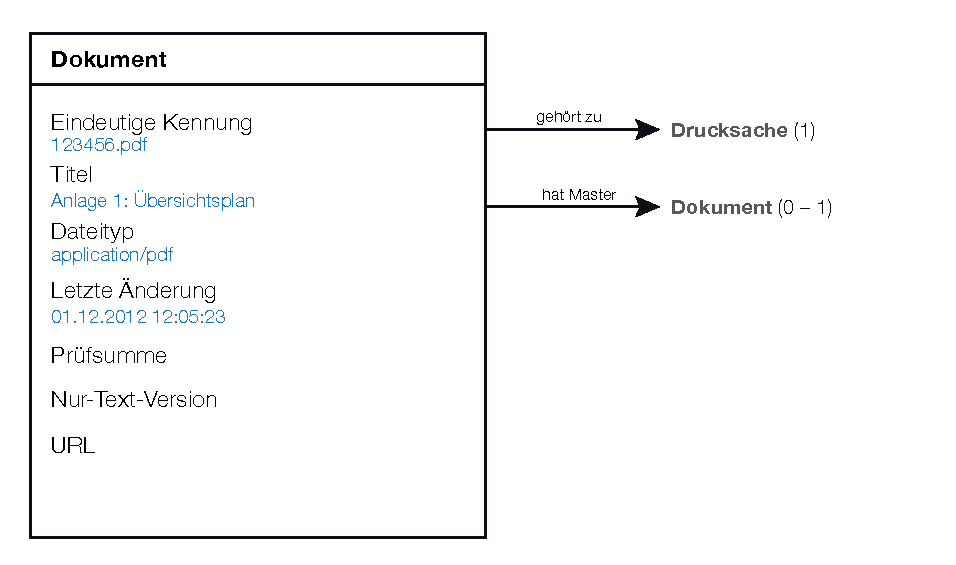
\includegraphics{images/datenmodell_dokument.pdf}
\caption{Objekttyp Dokument}
\end{figure}

\subsubsection{Eigenschaften}

\begin{description}
\item[Kennung]
Unveränderliche Kennung
\item[Titel]
Nutzerfreundliche Bezeichnung des Dokuments
\item[Dateityp]
Mime-Typ des Inhalts, z.B. ``application/x-pdf''
\item[Veröffentlichungsdatum]
Datum des Tages, an dem das Dokument ins System eingestellt wurde
\item[Änderungsdatum und -uhrzeit]
Datum und Uhrzeit der letzten Änderung des Dokuments
\item[Prüfsumme]
SHA1-Prüfsumme des Dokumenteninhalts
\item[Daten]
Der eigentliche (Binär-)Inhalt des Dokuments
\item[Nur-Text-Version]
Reine Text-Wiedergabe des Dokumenteninhalts, sofern es sich um ein
\end{description}

Textdokument handelt.

\subsubsection{Beziehungen}

\begin{itemize}
\item
  Dokumente gehören zwingend zu einer \textbf{Drucksache}, optional auch
  zu mehreren. Ein Dokument kann entweder als Hauptdokument einer
  Drucksache oder als Anlage eingestuft sein.
\item
  Ein Dokument kann auf ein anderes Dokument referenzieren, wenn es von
  dem anderen Dokument abstammt. So ist es möglich, von einem
  abgeleiteten Dokument zu seinem Dokumenten-Master zu gelangen
  (Beispiel: von einem PDF-Dokument zum OpenOffice-Original).
\end{itemize}

\subsection{Ort (\emph{location})}

Dieser Objekttyp dient dazu, einen Ortsbezug einer Drucksache formal
abzubilden. Ortsangaben können sowohl aus Textinformationen bestehen
(beispielsweise der Name einer Straße/eines Platzes oder eine genaue
Adresse) oder aus einer Geo-Koordinatenangabe aus Längen- und
Breitengrad.

Bislang finden sich nur beim Bonner System Beispiele für Ortsangaben.

\begin{figure}[htbp]
\centering
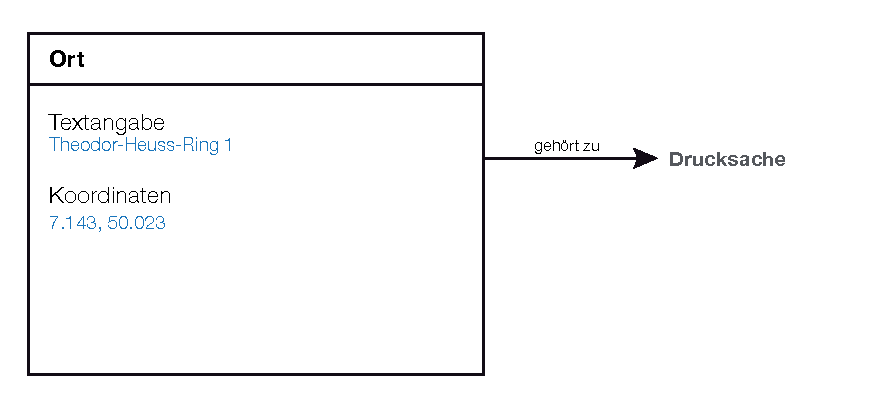
\includegraphics{images/datenmodell_ort.pdf}
\caption{Objekttyp Ort}
\end{figure}

\subsubsection{Eigenschaften}

\begin{description}
\item[Textanabe]
\emph{Optional.} Textliche Beschreibung eines Orts, z.B. in Form einer
Adresse
\item[Koordinaten]
\emph{Optional.} Längen- und Breitenangabe des Orts im WGS-84-System
{[}11{]}
\end{description}

\subsubsection{Beziehungen}

\begin{itemize}
\item
  Orte können mit Drucksachen in Verbindung stehen.
\end{itemize}

\section{Zugriffsmethoden}

In diesem Kapitel werden die Zugriffsmethoden der OParl-konformen
Schnittstelle beschrieben.

Stichpunkte:

\begin{itemize}
\item
  Grundlage für den Zugriff auf die Schnittstelle ist das Hypertext
  Transfer Protocol (HTTP).
\item
  Ausschließlich HTTP GET Methode
\item
  Optional gzip Encoding und andere Kodierungen, wenn Client und Server
  dies unterstützen
\item
  HTTP Last-Modified Header sowie Conditional GET sind bei Dateiabruf
  (Laden von Anhängen) zu unterstützen
\item
  Das Protkoll ist zustandslos
\item
  Authentifizierung wird nicht benötigt. Glossar =======
\end{itemize}

\begin{description}
\item[AGS]
Amtlicher Gemeindeschlüssel
\item[RIS]
Ratsinformationssystem
\item[WGS 84]
World Geodetic System 1984. Ein weltweites Referenzsystem für die
Interpretation von Geokoordinaten-Angaben.
\end{description}

\section{Fußnoten}

{[}1{]}: Siehe
\href{https://www.destatis.de/DE/Methoden/Klassifikationen/Bevoelkerung/StaatsangehoerigkeitGebietsschluessel.html}{www.destatis.de/\ldots{}}

{[}2{]}: Ratsinformationssystem der Stadt Köln,
\href{http://ratsinformation.stadt-koeln.de/}{http://ratsinformation.stadt-koeln.de/}

{[}3{]}: Firma Somacos,
\href{http://www.somacos.de/de/sitzungsdienst/ratsinfo.html}{SessionNet
Produktinformation}

{[}4{]}: Ratsinformationssystem der Bezirksverwaltugn Berlin Mitte,
\href{http://www.berlin.de/ba-mitte/bvv-online/allris.net.asp}{http://www.berlin.de/\ldots{}}

{[}5{]}: CC e-gov GmbH, \href{http://www.cc-egov.de/allris.htm}{ALLRIS
Produktionformationen}

{[}6{]}: Ratsinformationssystem der Stadt Rösrath,
\href{http://212.227.97.55/ratsinfo/roesrath}{http://212.227.97.55/\ldots{}}

{[}7{]}: \href{http://www.provox.de/}{Firma PROVOX}

{[}8{]}: Ratsinformationssystem der Stadt Euskirchen,
\href{https://sitzungsdienst.euskirchen.de/}{https://sitzungsdienst.euskirchen.de/}

{[}9{]}: Firma Sternberg,
\href{http://www.sitzungsdienst.net/produkte/ratsinformationsmanagement}{SD.NET
RIM Produktionformationen}

{[}10{]}: BoRis, Ratsinformationssystem der Stadt Bonn
(Eigenentwicklung).
\href{http://www2.bonn.de/bo\_ris/ris\_sql/agm\_index.asp}{http://www2.bonn.de/\ldots{}}

{[}11{]}: World Geodetic System 1984 (EPSG:4326), wird unter anderem
auch vom Global Positioning System (GPS) verwendet.

\end{document}
